\section{Implementation}
\label{netqasm:sec:implementation}

\subsection{Interface between \ac{CNPU} and \ac{QNPU}}
Here we explain the flow of messages between the \ac{CNPU} and the \ac{QNPU}.
The \ac{CNPU} starts by declaring the registration of an application, including resource-requirements for the application.
After this, the \ac{CNPU} sends some number of subroutines for the \ac{QNPU} to execute before declaring the application is finished.
See \cref{fig:message_sequence} for a sequence diagram and below for a definition of the messages.
In \cref{netqasm:sec:language} we will describe in more details the content of the subroutines and the format of instructions.
The \ac{QNPU} returns to the \ac{CNPU} an assigned application ID for the registered application and returns data based on the subroutines executed.

The \ac{CNPU} and the \ac{QNPU} are assumed to run independently and in parallel.
For example, while a subroutine is being executed by the \ac{QNPU}, the \ac{CNPU} could in principle do other operations, such as heavy processing or communication with another node.

\begin{figure}
      \centering
      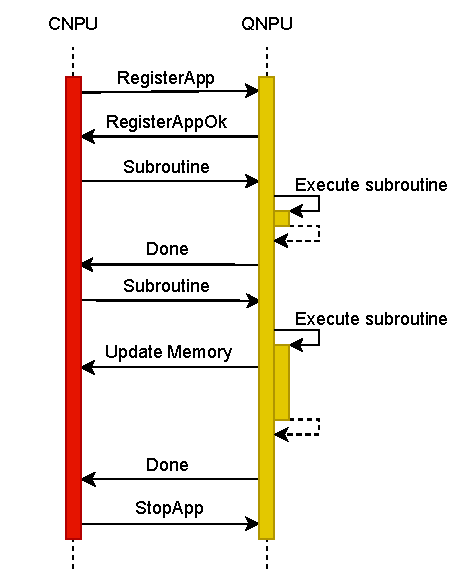
\includegraphics[width=0.5\linewidth]{figures/netqasm/message-flow.pdf}
      \caption{Flow of messages between the \ac{CNPU} and the \ac{QNPU}.}
      \label{fig:message_sequence}
\end{figure}

\Cref{fig:message_sequence} shows an example of a message exchange between the \ac{CNPU} and the \ac{QNPU}.
The content of these messages is further detailed in~\cref{netqasm:sec:app-messages}.



\subsection{The language}
\label{netqasm:sec:language}
The syntax and structure of \ac{NetQASM} resemble that of classical assembly languages, which in turn inspired the various QASM-variants for quantum computing~\cite{cross2017openqasm, khammassi2018cqasm, fu2019eqasm, liu2017fqasm}.

A \ac{NetQASM}-instruction is formed by an instruction name followed by some number of operands:
\begin{nqcode}
      instr operands
\end{nqcode}
where \nq{instr} specifies the instruction, for example \nq{add} to add numbers or \nq{h} to perform a Hadamard.
The \nq{operands} part consists of zero or more values that specify additional information about the instruction, such as which qubit to act on in the case of a gate instruction.
Instructions and operands are further specified in~\cref{netqasm:sec:operands}.

\subsection{Instructions}
\label{netqasm:sec:instructions}
There are eight groups of instructions in the \textbf{core} of \ac{NetQASM}.
Also summarized in \cref{fig:instructions}, these are:
\begin{itemize}
      \item \textbf{Classical:} Classical arithmetic on integers.
      \item \textbf{Branch:} Branching operations for performing conditional logic.
      \item \textbf{Memory:} Read and write operations to classical memory (register and arrays).
      \item \textbf{Allocate:} Allocation of qubits and arrays.
      \item \textbf{Wait:} Waiting for certain events. This can for example be the event that entanglement has been generated by the network stack.
      \item \textbf{Return:} Returning classical values from the \ac{QNPU} to the \ac{CNPU}.
            In our implementation we implement this by having the \ac{QNPU} write to the shared memory so that the \ac{CNPU} can access it.
      \item \textbf{Measurement:} Measuring a qubit.
      \item \textbf{Entanglement:} Creating entanglement with a remote node using the quantum network stack.
\end{itemize}

\begin{figure}
      \centering
      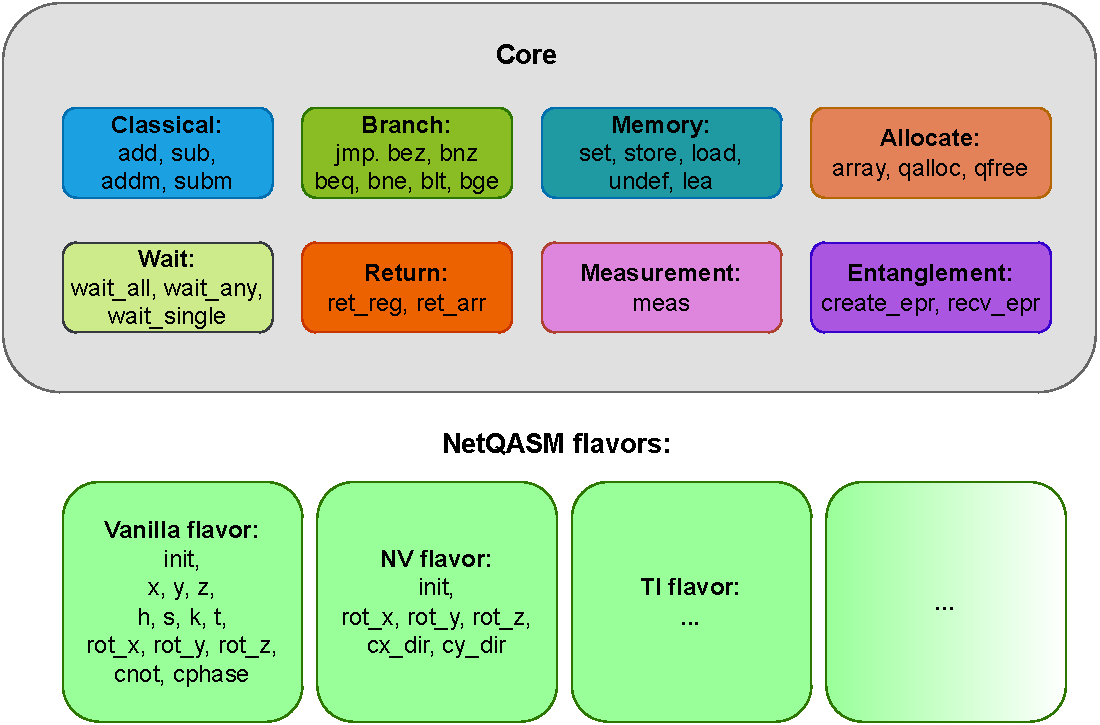
\includegraphics[width=0.8\linewidth]{figures/netqasm/instructions.pdf}
      \caption{The \textbf{core} of \ac{NetQASM} consists of eight groups of
            instructions. The quantum gates are defined as a set of software-visible
            gates part of a \ac{NetQASM} \textbf{flavor}. The \textbf{vanilla flavor}
            is the unique platform-independent \ac{NetQASM} \textbf{flavor} of
            \ac{NetQASM}, which can be used by a compiler.}\label{fig:instructions}
\end{figure}

Quantum gates are specific to a \ac{NetQASM} \textbf{flavor} and given as a set of software-visible gates of a given platform, see \cref{netqasm:sec:design_considerations}.
There is a single platform-independent \ac{NetQASM} \textbf{flavor} which we call the \textbf{vanilla flavor}, see \cref{fig:instructions}.
The \textbf{vanilla flavor} can be used as an intermediate representation for a compiler.


\subsection{Compilation}
Although application programmers could write \ac{NetQASM} subroutines manually, and let their (classical) application code send these subroutines to the \ac{QNPU}, it is useful and more user-friendly to be able to write quantum internet applications in a higher level language, and have the quantum parts compiled to \ac{NetQASM} subroutines automatically.
For this, we use the compilation steps depicted in \cref{fig:comp_chain}.
The format and compilation of the higher-level programming language is not part of the \ac{NetQASM} specification.
However, we do provide an implementation in the form of an SDK, see \cref{netqasm:sec:python-sdk}.

\begin{figure*}
      \centering
      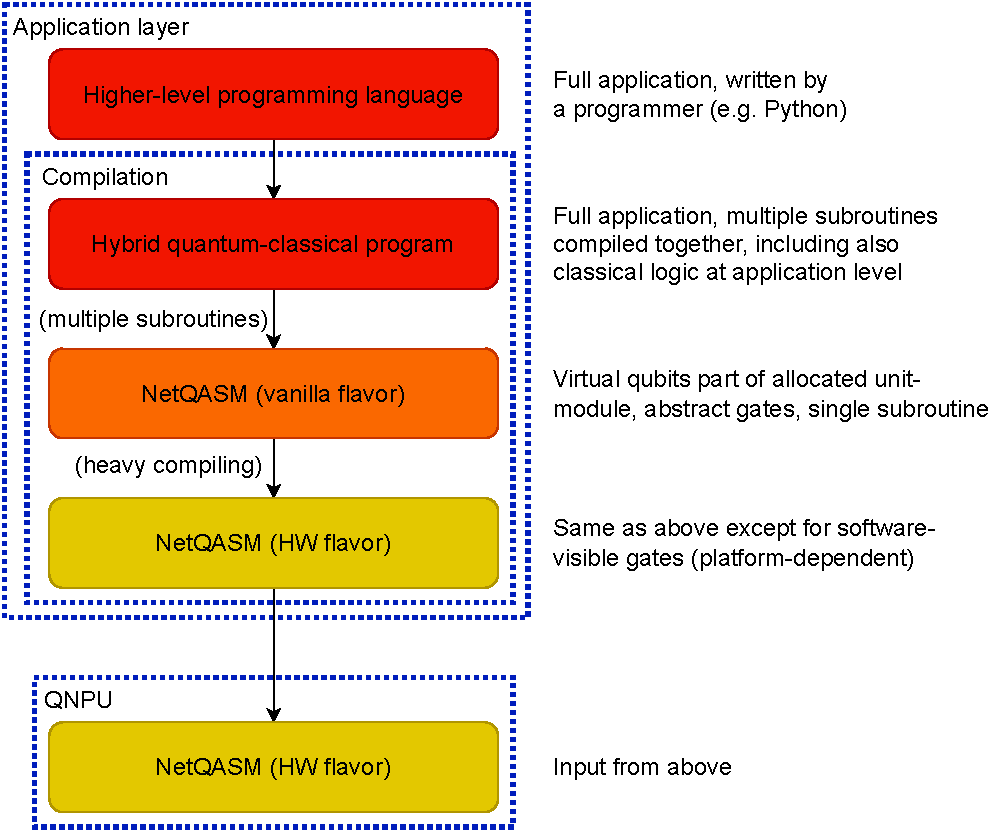
\includegraphics[width=0.7\linewidth]{figures/netqasm/comp-chain.pdf}
      \caption{Compilation steps from higher-level programming language, to the
            \ac{NetQASM} \textbf{flavor} exposed by the specific platform. What is
            contained at each level is further specified to the right of the
            diagram.}
      \label{fig:comp_chain}
\end{figure*}
